
\documentclass[preprint,12pt]{elsarticle}

\usepackage[spanish]{babel}
\usepackage{amssymb}
\usepackage{graphicx}
\usepackage{lineno}
\usepackage[utf8]{inputenc}
\usepackage{url}
\usepackage{natbib}

\begin{document}
	
	\begin{frontmatter}

		\title{\huge  PROYECTO DE  ANALISIS Y  MEJORAMIENTO DE  SOFTWARE }
		\author{Yaneth Virginia Aquino Huallp                (2017059286)}
		\author{Jesus Alejandro Quenaya Buiza              (---)}
		\author{Daniel Angel Juarez Chumpe              (---)}
		\address{Tacna, Perú}
		


%%INICIO abstract
\begin{abstract}
Con el presente documento se pretende presentar de forma concisa y clara las necesidades del cliente en el área a de ventas en términos de software que se realizará. 
En esta documentación se plasmará los requerimientos que servirán de guía para desarrollar el software en sus distintas etapas, ayudándonos a validar e inspeccionar la construcción de este, aplicando la calidad de Software.
Por ello se trabajara con  Sonarqube para el análisis de código estático
para analizar el código y encontrar errores de código, y vulnerabilidades de seguridad. 
El análisis C char de SonarSource tiene una gran cobertura de estándares de calidad bien establecidos.  
\end{abstract}
%%FIN abstract


\end{frontmatter}
%%INICIO Introducción
\section{Antecedentes oIntroducción}

El sistema de "SysFerreteria" esta desarrollado para poder automatizar los procesos que
normalmente realiza de forma manual, esto para llevar un correcto control del
inventario, compras a proveedores y ventas que se realizan a diario a los clientes;Además, implementar la emisión de Comprobantes de Pago para  los clientes.
%%FIN Introducción

%%INICIO Titulo
\section{Sistema de Ferreteria}
Propuesta de un sistema de facturación de  compra y venta
de artículos de ferretería.
%%FIN Titulo
%%INICIO Autores
\section{Autores}
\begin{itemize}
    \item Yaneth Aquino Huallpa
    \item Jesus Alejandro Quenaya Buiza  
    \item Daniel Angel Juarez Chumpe
\end{itemize}
%%FIN Autores
%%INICIO Planteamiento del problema
\section{Planteamiento del problema}
En la actualidad, para las empresas resulta una obligación llevar un mejor control y resguardo
de la información ya que de ésta depende, en su mayoría, el aumento o disminución de sus
ganancias o, a su vez, permite que las gestiones realizadas por sus trabajadores sean lo más
eficientes y óptimas para de ésta manera lograr los resultados esperados.

%%----------------------------------------------------------------------------------------------------------------------------------------------------------
	\subsection{\textbf{Problema}}
 En la microempresa “sysferreteria” ningún proceso se encontraba automatizado, todas
las actividades se realizaban manualmente y no se lograban concretar los procesos debido a la
magnitud de los mismos; por tal razón se procederá a desarrollar el sistema que contará con
módulos de usuarios, módulo de facturación, módulo de compras, gestión de inventario, módulo
de consultas y la generación de reportes que cumplan con los requerimientos de los usuarios
 y términos.
%%-----------------------------------------------------------------------------
	\subsection{\textbf{Justificación }}
Con el  presente proyecto  se pretende desarrollar el sistema de facturación para que de ésta forma el propietario conozca exactamente las ganancias netas diarias o mensuales
dependiendo de la necesidad que se tenga; además la falta de gestión del inventario impide al
usuario conocer las cantidades exactas de los productos que mantiene, su costo real y si es
necesario o no realizar pedidos en los tiempos determinados.

%%-----------------------------------------------------------------------------
	\subsection{\textbf{ Alcance }}
El software a desarrollar se basará en el área de ventas de la empresa, usando también el stock de los productos por lo cual:
El sistema permitirá registrar, actualizar, buscar y dar por “deteriorado” la información de los productos en stock. 
El sistema realizará ventas la cual nos permitirá agregar productos a la venta, restar con el stock, registrar o anular venta. 
El sistema permitirá añadir pedido (datos del producto y del cliente), registrar o anular pedido y listar pedidos.
El sistema permitirá generar reportes sobre: Ventas del día con el total ganado y Lista de Pedidos.
El sistema permitirá realizar la autentificación de los usuarios.


\section{Objetivos}
		\subsection{\textbf{ General }}
	 \begin{itemize}
		\item Desarrollar un software enfocado en el área de compra y ventas de la microempresa.
	 \end{itemize}
		\subsection{\textbf{Específicos }}
\begin{itemize}
	\item El sistema permitirá registrar, actualizar, buscar y dar por “deteriorado” la información de los productos en stock.
	\item El sistema realizará ventas la cual nos permitirá agregar productos a la venta, restar con el stock, registrar o anular venta. 
	\item El sistema permitirá añadir pedido (datos del producto y del cliente), registrar o anular pedido y listar pedidos. 
	\end{itemize}

	\section{Referentes teóricos}
\begin{itemize} 
    \item Hemos realizado una investigación en empresas relacionadas con el rubro de la ferretería, en este caso elegimos el caso de la empresa HELEO situada en el parque industrial de Tacna, donde pudimos observar como trabaja su sistema de COMPRA Y VENTA de productos.
	\begin{center}
	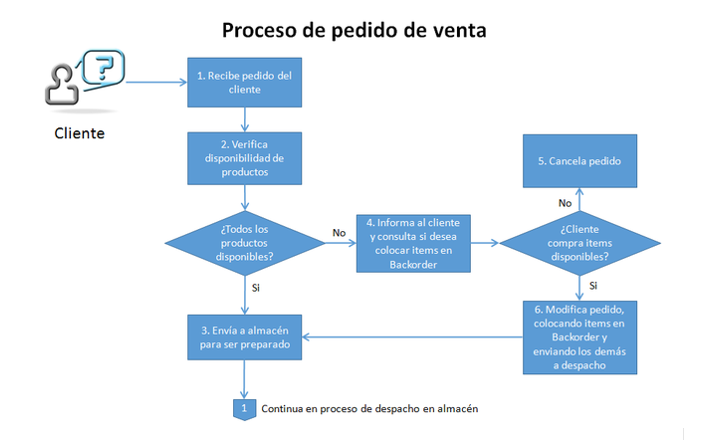
\includegraphics[width=12cm]{./imagen/1} 
	\end{center}
	\item Posee un anexo en la web de CATALOGO EN LINEA donde da una mayor promoción a sus productos antes de acudir a la tienda a comprarlos.
	\begin{center}
	
\includegraphics[width=12cm]{./imagen/2} 
	\end{center}
	\item Asimismo pudimos ver un detalle interesante que era un modulo de CONSULTA DE FACTURAS ELECTRONICAS VIA INTERNET para los clientes
	\begin{center}
	
\includegraphics[width=12cm]{./imagen/3} 
	\end{center}
\end{itemize}

\section{Desarrollo de la propuesta}
La calidad de código suele decirse que es un atributo interno de calidad, dado que no se hace visible al usuario. Pero llega un momento en el cual este atributo de calidad pasa de ser interno a externo, y esto se da cuando el hecho de tener modificar el código para hacer un cambio lleva mucho más tiempo del que debería. Con el fin de verificar la calidad interna de un sistema se suelen hacer análisis de código con SonarQube o herramientas similares. En este documento se muestra parte de de nuestro proyecto , donde básicamente  cuenta cómo hacer una prueba de concepto rápidamente usando una imagen Docker de SonarQube, y ejecutando el análisis desde SonarQube Scanner.
SonarQube, como tantas otras herramientas similares, permite realizar análisis estático de código fuente de manera automática, buscando patrones con errores, malas prácticas o incidentes. Además, realiza un cálculo de la deuda técnica. Dentro de las verificaciones que hacen herramientas como SonarQube, se encuentran las siguientes:
\begin{itemize}
	\item Detección de código duplicado..
	\item Falta de pruebas unitarias, falta de comentarios. 
	\item Código spaghetti, complejidad ciclomática, alto acoplamiento.
	\item Tamaño de archivos de código.
	\item Tamaño de métodos.
	\item No adecuación a estándares y convenciones de código.
	\item Vulnerabilidades conocidas de seguridad.
	
	Una muestra en Nuestro proyecto:
		
        \begin{center}
	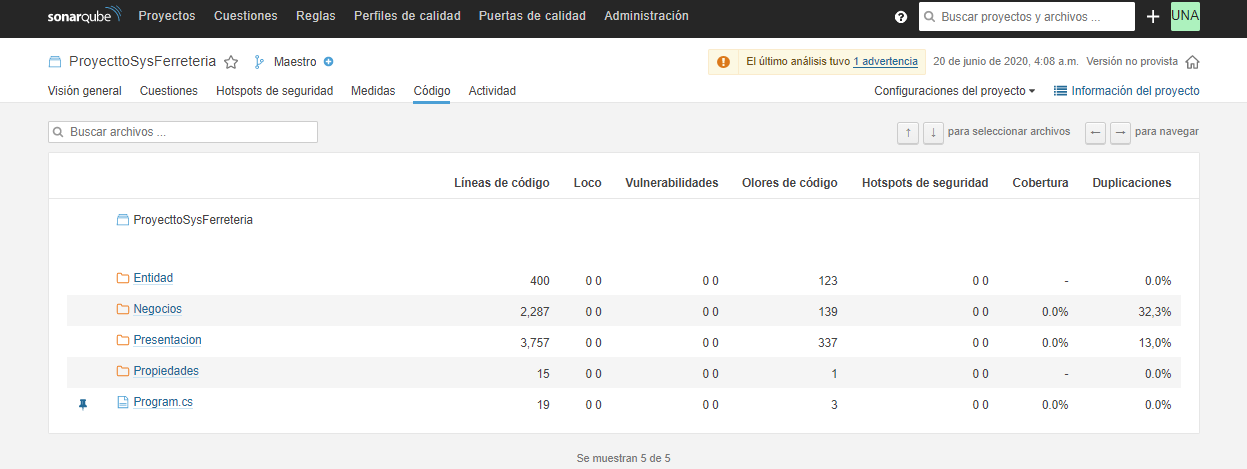
\includegraphics[width=12cm]{./imagen/7} 
	\end{center}
\end{itemize}

\subsection{\textbf{Tecnología de información  }}
		\begin{itemize}
	\item 	SQL SERVER: Microsoft SQL Server es un sistema de gestión de base de datos relacional, desarrollado por la empresa Microsoft. El lenguaje de desarrollo utilizado es Transact-SQL, una implementación del estándar ANSI del lenguaje SQL, utilizado para manipular y recuperar datos, crear tablas y definir relaciones entre ellas..
	\item 	C char : lenguaje de programación multiparadigma desarrollado y estandarizado por Microsoft. Es un lenguaje de programación creado para diseñar aplicaciones en la plataforma.NET.
	\item 	Visual Studio: es un entorno de desarrollo en diferentes sistemas operativos y compatibles con múltiples lenguajes de programación al igual que entornos de desarrollo web. 
	\end{itemize}
\subsection{\textbf{ Metodología, técnicas usadas  }}
UML es un lenguaje para hacer modelos y es independiente de los métodos de análisis y diseño. Existen diferencias importantes entre un método y un lenguaje de modelado. Un método es una manera explícita de estructurar el pensamiento y las acciones de cada individuo. Además, el método le dice al usuario qué hacer, cómo hacerlo, cuándo hacerlo y por qué hacerlo; mientras que el lenguaje de modelado carece de estas instrucciones. Los métodos contienen modelos y esos modelos son utilizados para describir algo y comunicar los resultados del uso del método.
          \begin{center}
	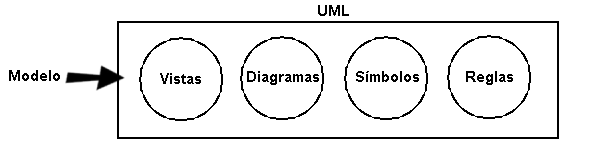
\includegraphics[width=12cm]{./imagen/5} 
	\end{center}
		
\section{Cronograma }

	\begin{center}
	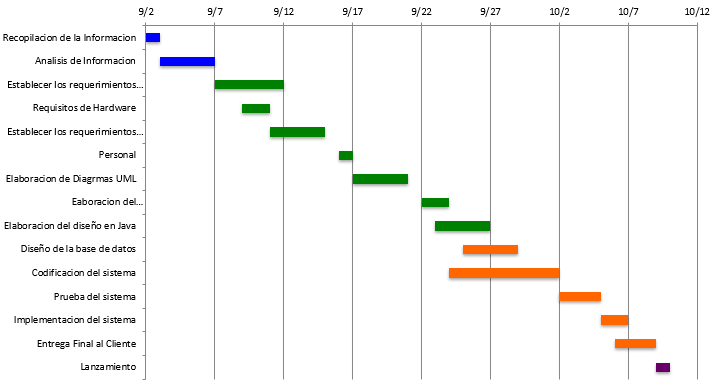
\includegraphics[width=12cm]{./imagen/20} 
	\end{center}

\section{Resultado Sonarqube}
	Definición de métricas
	\begin{itemize}
	    \item Código duplicado
	\begin{center}
	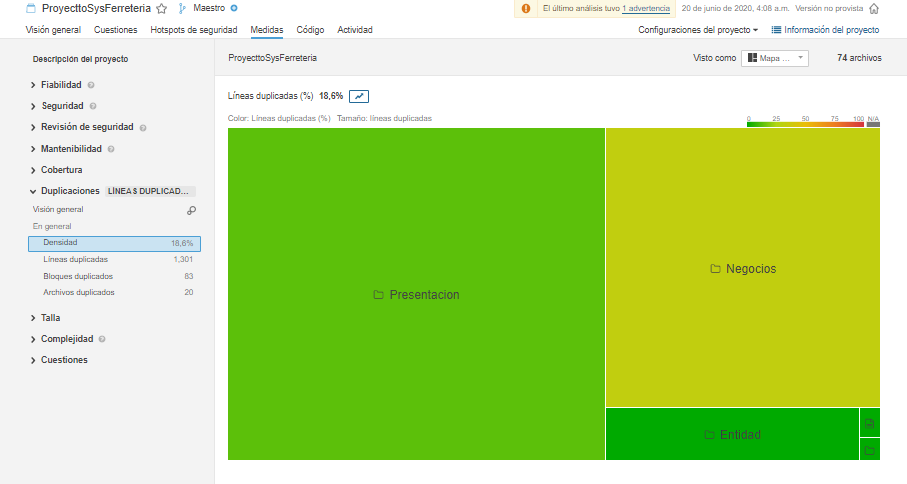
\includegraphics[width=12cm]{./imagen/8} 
	\end{center}
	\item Mantenibilidad
	\begin{center}
	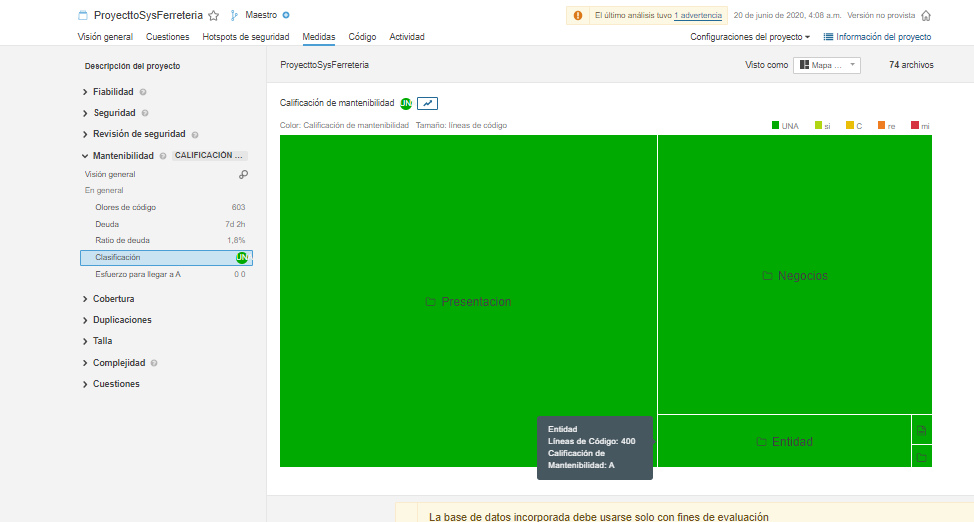
\includegraphics[width=12cm]{./imagen/9} 
	\end{center}
	\item Medida
		\begin{center}
	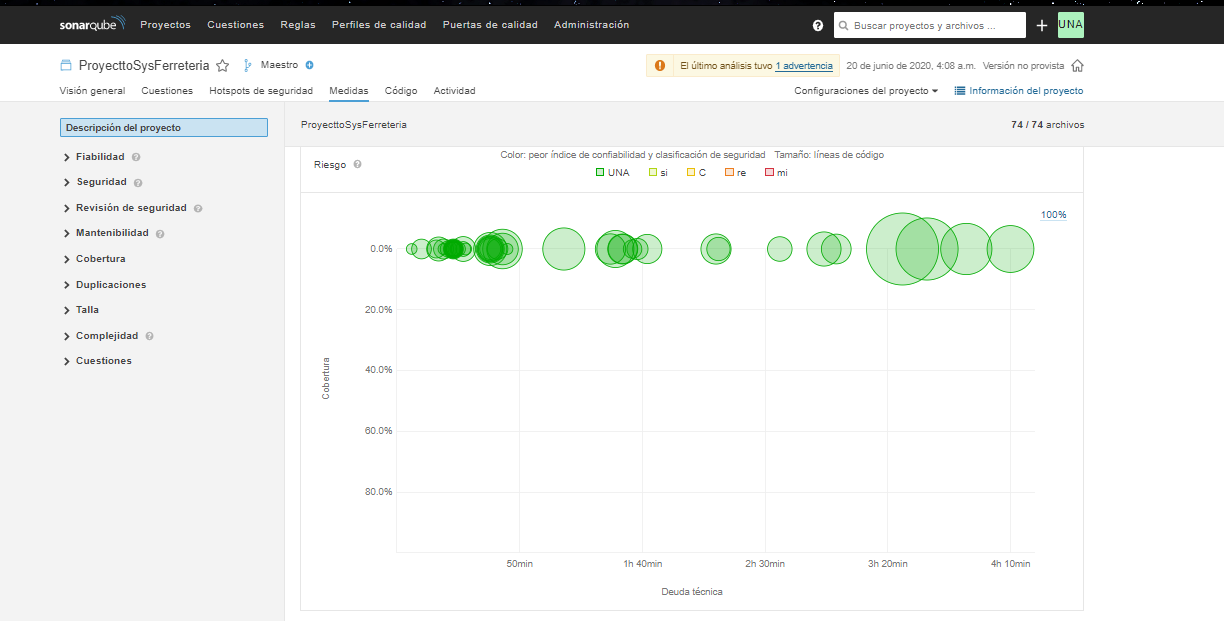
\includegraphics[width=12cm]{./imagen/10} 
	\end{center}
	\end{itemize}
\section{Desarrollo de Solución de Mejora}
\subsection{\textbf{ Casos de Uso de la aplicación}}
\begin{center}
	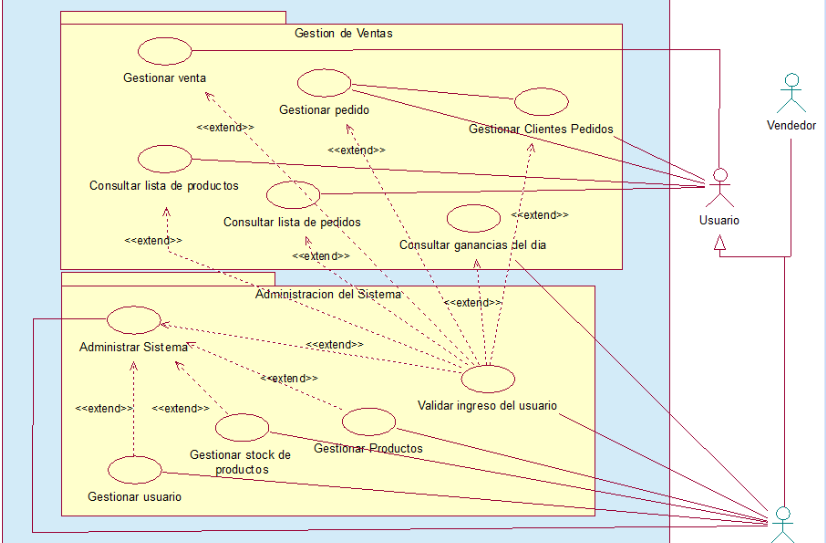
\includegraphics[width=12cm]{./imagen/casouso} 
	\end{center}
\subsection{\textbf{ Diagrama de Arquitectura de la aplicación }}



\begin{itemize}
\item Existen diferentes tipos de arquitectura o patrones a seguir para desarrollar un software, en este caso voy a explicar en que consiste la aqruitectura de 3 Capas , que ami parecer es la mas general o la mas basica para desarrollar.
	\item La Capa de Presentación : Donde se encuentran los formularios y la parte visual de la aplicación.
	\item 	La Capa de Negocios  : Donde se encuentra toda la logica del negocio y clases que las componete es decir, Entidades y controladoras)

	\item 	La Capa de Acceso a Datos: Donde se encuentra las conexiones y las transacciones que se utilizan para comunicarse con la base de datos.
	\end{itemize}
	\begin{center}
	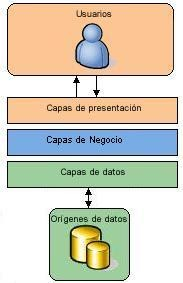
\includegraphics[width=7cm]{./imagen/capas} 
	\end{center}
	\begin{center}
	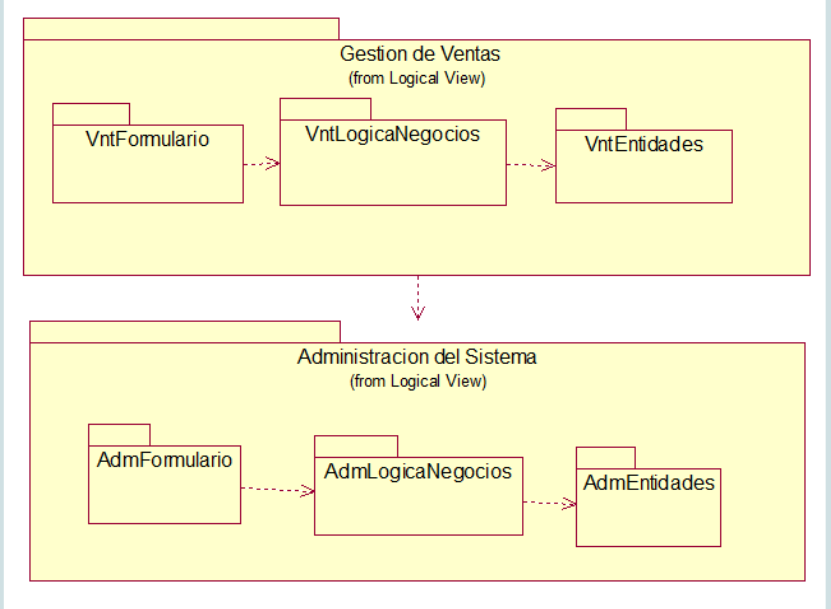
\includegraphics[width=12cm]{./imagen/vistalogica} 
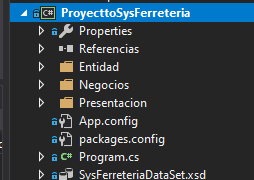
\includegraphics[width=7cm]{./imagen/3capas} 
	\end{center}
\subsection{\textbf{ Diagrama de Clases de la aplicación }}
\begin{center}
	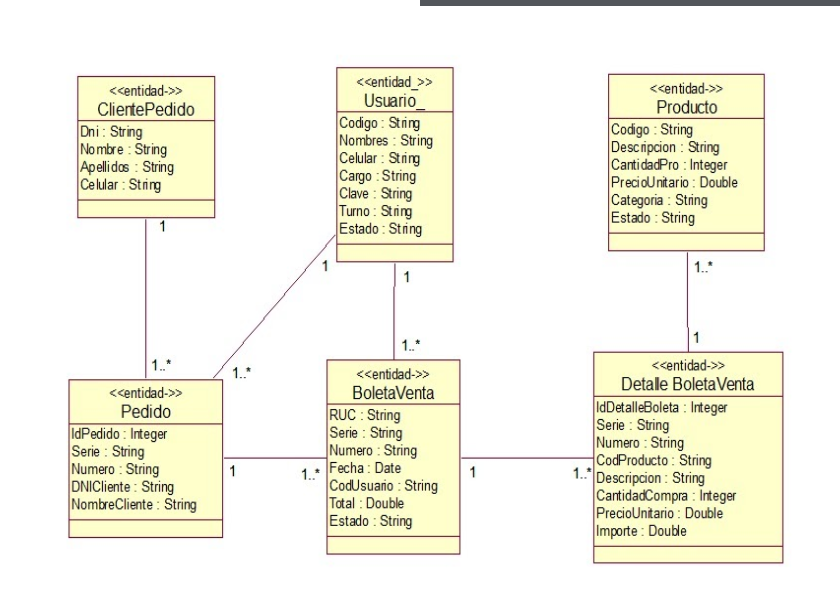
\includegraphics[width=12cm]{./imagen/diagrmclasesvistaprocesos} 
	
	\end{center}

\subsection{\textbf{  Metodos de pruebas implementados para coberturar la aplicación }}
\renewcommand{\labelenumi}{{\theenumi})}
\begin{enumerate}
\item  Pruebas Unitarias  
\begin{center}
	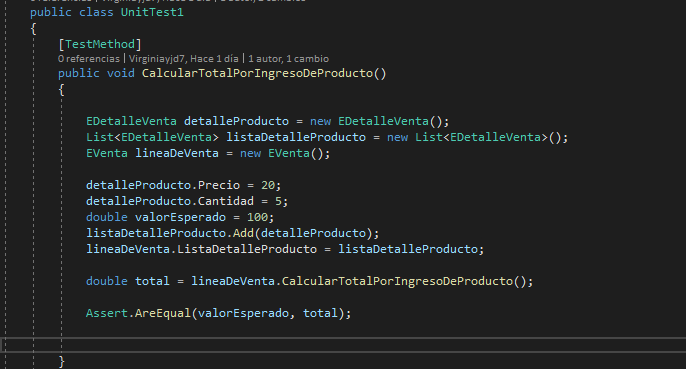
\includegraphics[width=12cm]{./imagen/calcular} 
	\end{center}
\begin{center}
	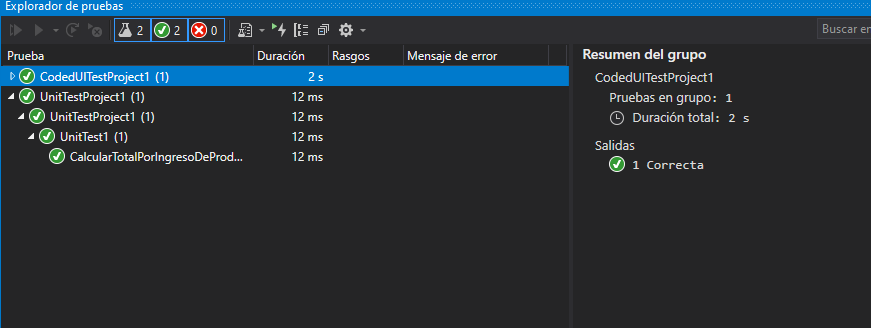
\includegraphics[width=12cm]{./imagen/pruebas} 
	\end{center}
\item  Pruebas de Interfaz 
\begin{center}
	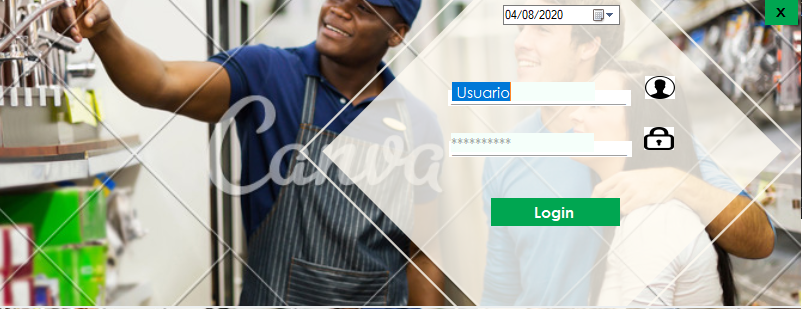
\includegraphics[width=12cm]{./imagen/interface} 
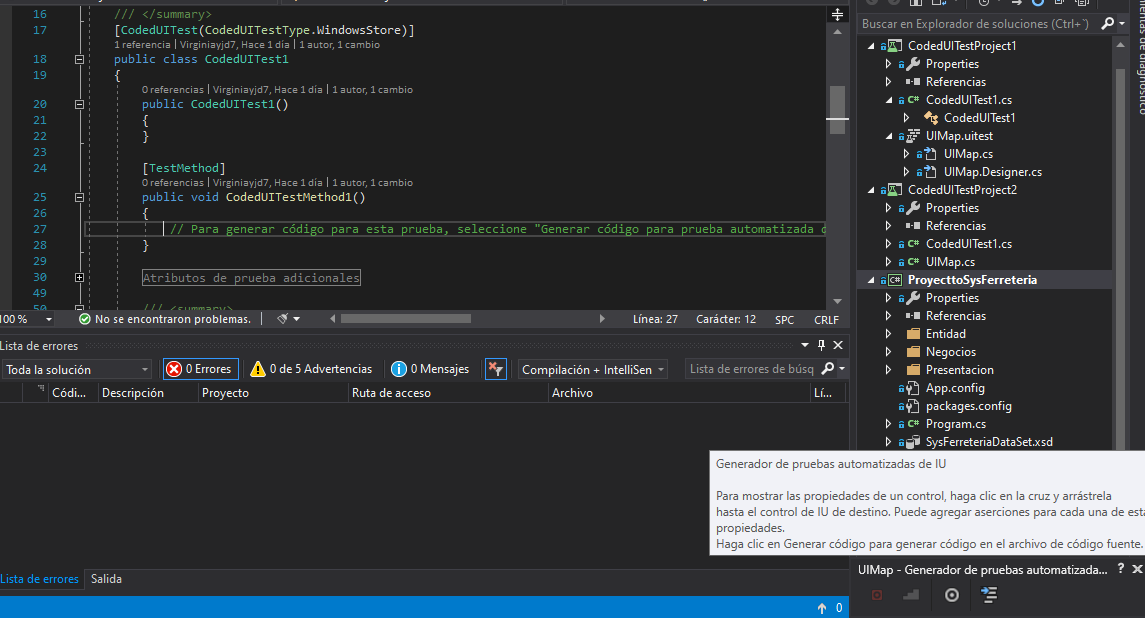
\includegraphics[width=12cm]{./imagen/f} 
	\end{center}
\item Pruebas basadas en Desarrollo Guiado por el Comportamiento
\end{enumerate}

	\newpage
	
	\bibliography{BIBLIOGRAFIA}	

\end{document}

